\documentclass{article}
\usepackage{pgfplots}
\pgfplotsset{compat=1.18}

\begin{document}

\begin{figure}[h]
\centering
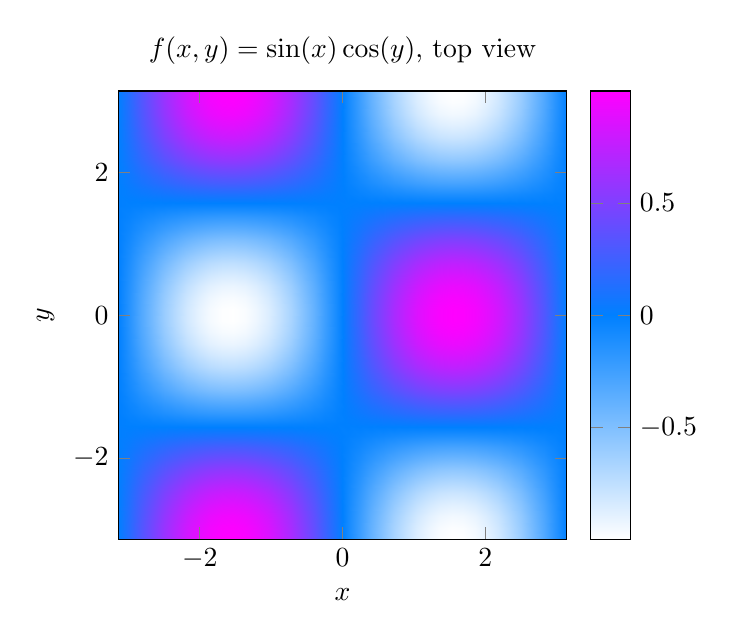
\begin{tikzpicture}
\begin{axis}[
    view={0}{90},
    xlabel={$x$},
    ylabel={$y$},
    colorbar,
    colormap/cool,
    title={$f(x,y) = \sin(x)\cos(y)$, top view},
    axis equal image,
]
\addplot3[
    surf,
    shader=interp,
    domain=-3.14:3.14,
    samples=40,
] {sin(deg(x))*cos(deg(y))};
\end{axis}
\end{tikzpicture}
\caption{Heat map of $\sin x \cos y$ seen from above.}
\end{figure}

\end{document}
